% `advanced_example.tex', an advanced example employing the AIAA class
% plus other third-party LaTeX packages.
%
% For a bare-bones usage, see `template.tex'.
%
% Typical processing for PostScript (PS) output:
%
%  latex advanced_example
%  bibtex advanced_example  (bibliography)
%  makeindex -s nomencl.ist -o advanced_example.gls advanced_example.glo
%                            (nomenclature)
%  latex advanced_example   (repeat as needed to resolve references)
%
%  xdvi advanced_example    (onscreen draft display)
%  dvips advanced_example   (postscript)
%  gv advanced_example.ps   (onscreen display)
%  lpr advanced_example.ps  (hardcopy)
%
% With the above, only Encapsulated PostScript (EPS) images can be used.
%
%
%  pdflatex advanced_example
%  bibtex advanced_example    (bibliography)
%  makeindex -s nomencl.ist -o advanced_example.gls advanced_example.glo
%                              (nomenclature)
%  pdflatex advanced_example  (repeat as needed to resolve references)
%
%  acroread advanced_example.pdf  (onscreen display)
%
% If you have EPS figures, you will need to use the epstopdf script
% to convert them to PDF because PDF is a limmited subset of EPS.
% pdflatex accepts a variety of other image formats such as JPG, TIFF,
% PNG, and so forth -- check the documentation for your version.
%
% If you do *not* specify suffixes when using the graphicx package's
% \includegraphics command, latex and pdflatex will automatically select
% the appropriate figure format from those available.  This allows you
% to produce PS and PDF output from the same LaTeX source file.
%
% To generate a large format (e.g., 11"x17") PostScript copy for editing
% purposes, use
%
%  dvips -x 1467 -O -0.65in,0.85in -t tabloid advanced_example
%
% For further details and support, read the Users Manual, aiaa.pdf.

\documentclass[]{aiaa-tc}% insert '[draft]' option to show overfull boxes

 \usepackage{varioref}%  smart page, figure, table, and equation referencing
 \usepackage{wrapfig}%   wrap figures/tables in text (i.e., Di Vinci style)
 \usepackage{threeparttable}% tables with footnotes
 \usepackage{dcolumn}%   decimal-aligned tabular math columns
  \newcolumntype{d}{D{.}{.}{-1}}
 \usepackage{nomencl}%   nomenclature generation via makeindex
  \makeglossary
 \usepackage{amssymb,amsmath}
 \usepackage{subfigure}% subcaptions for subfigures
 \usepackage{subfigmat}% matrices of similar subfigures, aka small mulitples
 \usepackage{fancyvrb}%  extended verbatim environments
 \fvset{fontsize=\footnotesize,xleftmargin=2em}
 \usepackage{lettrine}%  dropped capital letter at beginning of paragraph
%  \usepackage[dvips]{dropping}% alternative dropped capital package
 \usepackage[colorlinks]{hyperref}%  hyperlinks [must be loaded after dropping]
 \usepackage{float}
 \usepackage{longtable,booktabs,tabularx}
 % \restylefloat{table}
 \usepackage{graphicx}
 \usepackage{caption}
 \usepackage{siunitx}
 \usepackage{multicol}
 \usepackage{indentfirst}
 \usepackage{environ}
 \usepackage[labelfont=bf]{caption}
 \usepackage{multirow}
 \usepackage{setspace}
%  \graphicspath{{./figs/}}
 \usepackage[sort, numbers]{natbib}

\usepackage{bm}
%\title{Conceptual Design of an Extremely Short Takeoff and Landing Aircraft (using GPkit/for Urban Air Mobility)}
\title{Feasibility Study of Short Takeoff and Landing Urban Air Mobility Vehicles using Geometric Programming}
 \author{
  Chris Courtin\thanks{Graduate Student, Aeronautics and Astronautics Engineering, MIT, 77 Mass Ave, Cambridge MA, 02139, AIAA Member.}, 
  Michael Burton\thanks{Graduate Student, Aeronautics and Astronautics Engineering, MIT, 77 Mass Ave, Cambridge MA, 02139, AIAA Student.}, 
  Patrick Butler\thanks{Graduate Student, Aeronautics and Astronautics Engineering, MIT, 77 Mass Ave, Cambridge MA, 02139, AIAA Student.}, 
  Alison Yu\thanks{Graduate Student, Aeronautics and Astronautics Engineering, MIT, 77 Mass Ave, Cambridge MA, 02139, AIAA Student.}, 
 Parker Vascik \thanks{Graduate Student, Aeronautics and Astronautics Engineering, MIT, 77 Mass Ave, Cambridge MA, 02139, AIAA Student.}, 
  John Hansman\thanks{T. Wilson Professor, Aeronautics and Astronautics Engineering, MIT, 77 Mass Ave, Cambridge MA, 02139, AIAA Member.} \\
  {\normalsize\itshape
   Massachusetts Institute of Technology, Cambridge, 02139, USA}\\
 }

 % Data used by 'handcarry' option
 \AIAApapernumber{YEAR-NUMBER}
 \AIAAconference{Conference Name, Date, and Location}
 \AIAAcopyright{\AIAAcopyrightD{YEAR}}

 % Define commands to assure consistent treatment throughout document
 \newcommand{\eqnref}[1]{(\ref{#1})}
 \newcommand{\class}[1]{\texttt{#1}}
 \newcommand{\package}[1]{\texttt{#1}}
 \newcommand{\file}[1]{\texttt{#1}}
 \newcommand{\BibTeX}{\textsc{Bib}\TeX}
 \usepackage{hyperref}
 \hypersetup{citecolor = blue}

\begin{document}

\graphicspath{{./figs/}}
\maketitle

\begin{abstract}
    The feasibility of an Urban Air Mobility (UAM) system that features electric Extremely Short Takeoff and Landing (ESTOL) vehicles is investigated.  An overview is given of the system constraints that must be incorporated into the design of the vehicle.  The system-wide advantages and limitations of ESTOL aircraft are discussed, for both near- and far-term system implementations.  A detailed vehicle sizing model is developed using geometric programming, a robust optimization framework.  This model is used to determine feasible boundaries on required runway size, vehicle range, and the sensitivity of the vehicle design to high-level mission parameters such as speed and number of passengers.  Key unique drivers of the vehicle design are identified.  The impact of distributed electric propulsion (DEP) is assessed.  Performance relative to a comparable Vertical Takeoff and Landing (VTOL) vehicle is analyzed, both with currently available technology and forecasted future technology.   The infrastructure requirements (runway size, approach paths, etc.) needed to support ESTOL operations are assessed according to current regulations.  Two major urban areas (Boston and Los Angeles) are presented as case studies to show where this infrastructure could be feasibly located.  Key challenges and risks to implementation are discussed.  


\end{abstract}

\section*{Nomenclature}

\begin{multicols}{2}
\small

\begin{tabbing}
  XXXXXXX \= \kill% this line sets tab stop
$A$ \> takeoff helper variable \\
$AR$ \> wing aspect ratio \\
$b$ \> wing span \\ % [ft] \\
$B$ \> takeoff helper variable \\
$c$ \> wing chord \\ %[m] \\
$C_D$ \> drag coefficient \\
$CDA$ \> area drag coefficient \\
$C_{D_g}$ \> ground drag coefficient \\
$c_{d_p}$ \> wing profile drag coefficient \\
$C_L$ \> lift coefficient \\
$C_{L_g}$ \> ground lift coefficient \\
$C_{L_{\mathrm{max}}}$ \> max lift coefficient \\
$D$ \> drag \\
$e$ \> span efficiency \\
$f_{\mathrm{struct}}$ \> fractional structural weight \\
$g$ \> gravitational constant \\
$L$ \> lift \\
$\mathcal{M}_{\mathrm{root}}$ \> root moment stress \\
$N$ \> deceleration factor \\
$P_{\mathrm{shaft-max}}$ \> max shaft power \\
$P_{\mathrm{spec}}$ \> specific motor power \\
$Re$ \> Reynolds number \\
$S$ \> wing area \\
$S_{\mathrm{land}}$ \> landing ground roll \\
$S_{\mathrm{runway}}$ \> runway distance \\
$S_{\mathrm{TO}}$ \> take off ground roll \\
$S_{y_{\mathrm{spar}}}$ \> spar section modulus \\
$t$ \> time \\
$T$ \> thrust \\
$V$ \> speed \\
$V_{\mathrm{stall}}$ \> stall speed \\
$W_{\mathrm{batt}}$ \> battery weight \\
$W_{\mathrm{fadd}}$ \> additional wing weight\\
$W_{\mathrm{motor}}$ \> motor weight \\
$W_{\mathrm{MTO}}$ \> max take off weight \\
$W_{\mathrm{pay}}$ \> payload weight \\
$W_{\mathrm{skin}}$ \> wing skin weight \\
$W_{\mathrm{spar}}$ \> wing spar weight \\
$W_{\mathrm{struct}}$ \> structural weight \\
$W_{\mathrm{wing}}$ \> wing weight \\
$\eta_{\mathrm{elec}}$ \> combined electric efficiency \\
$\eta_{\mathrm{prop}}$ \> propeller efficiency \\
$\mu$ \> rolling friction coefficient \\
$\rho$ \> air density \\
$\sigma_{\mathrm{CFRP}}$ \> carbon fiber allowable stress \\
 \end{tabbing}

\end{multicols}
% \printglossary% creates nomenclature section produced by MakeIndex

\section{Introduction}
Urban Air Mobility (UAM) is a broad concept that refers to a set of related operations and technologies that aim to provide on-demand intra-city and regional air transportation.  UAM concepts of some form or another have been around for at least the past fifty years.  Helicopters have been performing UAM-type missions since the 1960s and have sufficient performance capability to meet nearly all payload, speed, and range requirements of the current UAM mission profile. However, historical helicopter public transportation networks by and large did not succeed and do not exist today due to the high costs of helicopter operation, the high noise generation of these vehicles, and the poor safety record of these aircraft.  Recently, advances in electric vehicle propulsion and key subsystem technologies has opened up the vehicle design space and enabled new approaches to mitigating some of these systemic challenges.  This has sparked renewed interest in the UAM concept and the development of UAM-specific vehicles.  Numerous legacy and emerging aircraft manufacturers are developing vehicles for this mission with novel configurations that leverage more-electric or all-electric vehicles and propulsion systems.  

Many different vehicle architectures are being developed, including multicopters, tilt-rotors, and slowed rotors.  While some utilize wing-borne lift for the cruise phase of flight every vehicle proposed to date has Vertical Takeoff and Land (VTOL) capability.  In almost all configurations, this is accomplished via a distributed electric propulsion (DEP) system of many small electric motor/propeller combinations.  VTOL capability minimizes the amount of space the vehicle requires to take off, and minimizes susceptibility to crosswinds, while DEP increases system efficiency and safety.  This is useful capability for operations in areas where space is at a premium, but imposes two significant penalties on the vehicle.  The first is in performance; the weight of the high-power system needed to perform the vertical takeoff and landing limits the amount of payload these vehicles can carry, or the range at which they can carry it.  This effect is especially pronounced for electric aircraft, where payload and range are already compromised by the poor specific energy of current battery technology relative to hydrocarbon fuels.  The second, and more significant,  penalty is that VTOL configurations increase the already substantial amount of risk associated with the UAM concept.  

Any proposed UAM system is exposed to many sources of risk, such as local noise regulations, ATC capacity concerns, pilot or automation availability, infrastructure availability, and uncertain market demand.  Of all the risk sources, perhaps the greatest is the FAA certification of these new types of aircraft.  This risk is so significant in part because historically, certification of new aviation technologies is a difficult process, and also because an inability to certify a vehicle would preclude UAM operations at any scale. 

For an electric VTOL (eVTOL) configuration to be certified, there must be a very small probability ($10^-7 - 10^-8$ according to the current standards) of a catastrophic failure per flight hour. In practice, this means that all key vehicle failure modes must be effectively mitigated.  In any distributed electric propulsion vehicle, there are three key failure modes - low altitude failure of the flight stabilization system, a low-altitude common mode power system failure, and a battery thermal runaway.  All DEP VTOL configurations rely on an active stabilization system for the vertical and transitional phases of flight; any failure of this system, or the power delivery system, cannot be tolerated, as it would result in a loss of vehicle control.  At high altitudes an airframe parachute is a possible mitigation but current ballistic recovery systems are only certified above 400ft AGL (or higher with no forward airspeed) ~\cite{parachutes}; during takeoff and landing they are not effective. These failure modes are difficult to mitigate, especially in highly weight- and cost-sensitive vehicles.  Precedent exists, in the form of triply-redundant, isolated systems like those found on commercial jetliners, but certification of those systems is a costly and difficult process.   

The risk of a lithium polymer battery going into thermal runaway is another key certification risk.  Thermal runaway is where a short circuit forms within the battery, causing an uncontrolled increase in temperature and pressure, which can trigger a chain reaction in neighboring cells.  There are several ways a battery cell could go into thermal runaway; over-charging or over-discharging, mechanical damage, or an internal short circuit caused by a manufacturing defect ~\cite{batteries}.  While modern battery control systems can effectively prevent over-charging of the battery, mechanical damage and especially internal short circuits are hard to prevent with a high degree of certainty.  Current regulations therefore require that flight batteries are shown to be safe in the event of a thermal runaway~\cite{other batteries}.  This regulation is normally complied with through battery containment, which adds potential significant weight to the battery system ~\cite{even more batteries}.  

The intention here is not to argue that it is impossible to certify an eVTOL aircraft, but rather to emphasize that it will be a difficult, expensive process which has a good chance of further penalizing already marginal vehicle performance.  Certification of any new aviation technology is hard, and combining multiple new technologies into a novel vehicle configurations adds risk to an already difficult process.  Since certification currently is a prerequisite for any commercial flight activity ~\cite{FARs}, this process will pace any proposed UAM network implementation.  

One way of reducing the certification risk which has not been widely considered is to use a lower-risk vehicle architecture that minimizes the amount of new technology required. One vehicle architecture which has not been widely considered for the UAM mission is the extremely short takeoff and land (STOL) aircraft, which are fixed-wing aircraft design primarily for short-field operations.  By utilizing the wing throughout all phases of flight, STOL aircraft have performance advantages compared to VTOL aircraft of similar payload capacity.  Since they are inherently stable, there is no need for electrically actuated controls or a flight stabilization system.  This eliminates the need for a complex control architecture and the associated redundant systems.  While an automated flight system may be desirable at some future point, initial operations of any configuration are expected to be piloted [probably say this earlier]; a vehicle could be certified without any capability.  If they are electrically powered, thermal runaway in the battery system is still a concern.  However, STOL configurations are less sensitive to weight than VTOL configurations, potentially lessening the performance penalty associated with a battery containment system. 

The clear downside of STOL aircraft is they require some length of runway, which increases the infrastructure required.  In dense urban areas, there availability of infrastructure is severely limited.  If no runways can be placed in useful locations, then all the other advantages of STOL vehicles are immaterial.  To realize those advantages, it must be possible to design an aircraft that can land on a runway short enough that there are a large number of potential locations in a dense urban area.  
The purpose of this paper is to conducts an in-depth analysis into the feasibility of an UAM system that features ESTOL aircraft, from both a vehicle and infrastructure perspective.  The goal is to determine how short a runway a fixed-wing aircraft with modern technology can be designed to land on, as well as the effects of runway length on potential locations in urban areas.  
To conduct the vehicle design trade studies, a geometric programming (GP) vehicle sizing and performance model is developed to rapidly and holistically consider the large design space.  Ground infrastructure and approach path constraints are internalized in this model as design constraints on the aircraft.  This model is exercised to determine feasible bounds on runway operating length, and how vehicle range, speed, and payload capacity trade with ground infrastructure requirements.  
To assess the ground infrastructure requirements, the current FAA guidance for airport design and approach path layouts is used to create the nominal layout for a short takeoff and landing area (STOLA).  The feasibility of locating these STOLA near major urban areas is assessed by looking at case studies of two particular cities, Boston and Los Angeles.  The potential for ESTOL aircraft to act as a pathway to the development of large-scale UAM systems is reviewed from a technical, operational and business feasibility perspective. Furthermore, the complementary nature of ESTOL aircraft operations and potential future VTOL UAM operations are hypothesized. As part of this work, previous literature concerning small aircraft transportation system design ~\cite{Viken}, ~\cite{Holmes}, thin-haul transportation vehicles ~\cite{Harish},~\cite{Kreimeier},~\cite{Justin} �, VTOL aircraft ~\cite{Duffy}, and STOL aircraft is considered ~\cite{Antcliff},~\cite{SeeleyIV}. 
 

\section{Key enabling technologies}


\paragraph{Current Technology} ESTOL aircraft are not a new concept.  The Helio Courier, first built in the late 1940s, is one existing example, with demonstrated takeoff and landing distances from 100-300ft.  Highly experienced bush pilots are able to achieve landing distances on the order of single aircraft lengths.  Developing an aircraft that can operate of extremely short runways is clearly technologically feasible.  Nevertheless, ESTOL aircraft technology has not found wide adoption outside of the relatively small community of pilots who routinely fly to remote, relatively unimproved landing areas.   There are inherent challenges in taking existing ESTOL aircraft and using them for operations near major urban areas, which are a result of the design penalties that ESTOL capability drove on the vehicles.  
For example, current ESTOL vehicles achieve their short field performance through a combination of low wing loading, high power-to-weight, and extensive use of high-lift systems.  The low wing loading means that both maximum and best cruise speeds are fairly low.  Additionally, it makes the vehicles highly sensitive to gusts and turbulence, an important consideration for passenger operations.   The high-lift systems required are also complex (except with very low wing loadings), which adds a weight and cost penalty to these vehicles.  Depending on the type of powerplant type used, the need for high power at takeoff may also reduce the efficiency at the nominal cruising point.  More significantly, these high-power engines generated substantial noise on takeoff; a primary consideration when operating near urban areas. 

\paragraph{Key Enabling Technologies} The introduction of new electric aircraft technologies has the potential to change the paradigm of current ESTOL aircraft and make them practical for use in an UAM setting.   In the case of an all-electric aircraft, the reduction in noise through the use of batteries and an electric motor is one key area of improvement.  Another is the use of blown lift with distributed electric propulsion, in a configuration similar to the NASA X-57 Maxwell.  This has the ability to generate very high effective lift coefficients (especially on takeoff), with a reduction in the complexity of the high-lift system required and/or an increase in the climb path angle.  This technology allows in increase in the vehicle wing loading, which improves the cruising speed and passenger comfort.  
Additionally, since electric motors can be run above their maximum rated capacity for short periods of time, the weight penalties of installing a high-thrust system that is only needed on takeoff are reduced.  And since most of the motors would be shut down in cruising flight, the propulsion system can be designed to operate at or near peak efficiency throughout most of the mission.  When taken together, these key technologies enable the design of a practical ESTOL vehicle.  The range limitations come mostly from the use of batteries and their poor specific power relative to hydrocarbon fuels; replacing them with a hybrid-electric system could extend the range or reduce vehicle takeoff weight, with associated tradeoffs on noise, emissions, and direct operating cost.  

\\-DEP
\\-Blown Lift
	-Limited utility on approach. Cite NASA paper with same considerations
\\-High power electric motors
	-Power burst
	-Braking
\\-Deceleration methods/limits
\\-Advanced flight controls 
	-Post stall landings
	-Advanced approach guidance

\\Technology summary table. 
\\-Baseline vs advanced technology
\\-Baseline technology is simplest instantiation of concept
\\-Advanced technology increases performance and risk 
 


\section{Market Analysis}

[Assert our market case for stol aircraft; 
\\-commuting most pressing use case. 
\\-Large commuting populations live within 100 nmi of major metro areas. 
\\-Surface congestion extends at least 50nmi.  
\\-100 nmi provides useful capability; speed must be faster than a car - 100kts nominal. 
\\-Widespread existing air infrastructure in surrounding region, relatively low barriers to construction
\\-Lack of existing infrastructure in major urban centers.
\\-Need to build substantial infrastructure in city center. - This should be a high near-term risk on chart.  ]
\\-This is in line with other analyses of this market space - NASA, Uber, Joby

\section{Vehicle Feasibility}

A sizing study using Geometric Programming optimization was performed to understand how vehicle performance and design would be effected by short take offs and landings. 
This section describes the assumptions and equations used in the optimization model for vehicle size, cruise performance, and takeoff and landing distances.

Geometric programming was selected as a means of evaluating this trade space because of its speed and reliability.  
Geometric programming is a special type of convex, non-linear optimzation.\cite{gp}
Because it is convex, even GPs with thousands of variables can be solved quickly.\cite{gp}
Additionally, recent research has shown that GPs can be used to evaulate aircraft design trade spaces.\cite{burton_solar_2017}\cite{gpkit}


\subsection{Vehicle Model}

It is assumed that the aircraft is completely electric, replying on battery power for powered flight. 
The aircraft weight is comprised of the battery, payload, wing, motor, and structural weight,

\begin{equation}
    W_{\mathrm{MTO}} \geq W_{\mathrm{batt}} + N_{\mathrm{pax}}W_{\mathrm{pax}} + W_{\mathrm{wing}} + W_{\mathrm{motor}} + W_{\mathrm{struct}}
\end{equation}

where the motor, passenger, and structural weights are

\begin{align}
    W_{\mathrm{motor}} &\geq \frac{P_{\mathrm{shaft-max}}}{P_{\mathrm{spec}}} \\
    W_{\mathrm{pax}} &= 195 \mathrm{[lbf]} \\
    W_{\mathrm{struct}} &\geq W_{\mathrm{MTO}}f_{\mathrm{struct}}.
\end{align}

The battery weight is constrained by the range of the aircraft

\begin{equation}
    R \leq \frac{h_{\mathrm{batt}} W_{\mathrm{batt}} \eta_{\mathrm{elec}} V}{gP_{\mathrm{shaft}}}
\end{equation}

where the shaft power is 

\begin{equation}
    P_{\mathrm{shaft}} \geq \frac{TV}{\eta_{\mathrm{prop}}}
\end{equation}

The aircraft is assumed to be in steady level flight during cruise. 

The wing weight is composed of the skin, main spar and additional components

\begin{equation}
    W_{\mathrm{wing}} \geq W_{\mathrm{skin}} + W_{\mathrm{spar}} + W_{\mathrm{fadd}}
\end{equation}

The skin and structural elements are assumed to be carbon fiber.  
The wing spar configuration is a cap spar with unidirectional carbon fiber caps wrapped in a shear web as shown in Figure~\ref{f:capspar}.  

\begin{figure}[h!]
	\begin{center}
	\includegraphics[width=0.9\textwidth]{capspar.pdf}
    \caption{\textbf{Cross sectional view of a cap spar.}}
	\label{f:capspar}
	\end{center}
\end{figure}

The spar dimensions are sized such that the material stresses are not exceeded under a 3.5 g-load,

\begin{equation}
    \sigma_{\mathrm{CFRP}} \geq \frac{\mathcal{M}_{\mathrm{root}}}{S_{y_{\mathrm{spar}}}}
\end{equation}

The root wing moment $\mathcal{M}_{\mathrm{root}}$, is calculated assuming a distributed load along the wing span that scales with the local chord.\cite{bending}
A constant tapered wing is assumed.  
This wing sizing model leverages the GP wing sizing model used by Burton and Hoburg.\cite{burton_solar_2017} 

A simple drag model is used for the aircraft, 

\begin{equation}
    C_D \geq CDA + c_{d_p} + \frac{C_L^2}{\pi e AR}.
\end{equation}

where the profile drag coefficient $c_{d_p}(C_L, Re)$, is calculated from a representative wing polar. 
The combined drag and wing loading models allow the aspect ratio to be optimized, trading structural integrity with aerodynamic performance. 

\subsection{Takeoff and Landing Models}

The takeoff model was adapted from Raymer's takeoff equations to fit a GP compatible form.  Using equations of motion the takeoff state can be expressed

\begin{equation}
    T - D - \mu(W_{\mathrm{MTO}} - L) = \frac{W_{\mathrm{MTO}}}{g} \frac{dV}{dt}.
\end{equation}

This can be simplified to 
\begin{align}
    \frac{dV}{dt} &= g \left( \frac{T}{W_{\mathrm{MTO}}} - \mu \right) - \frac{g}{W_{\mathrm{MTO}}} \left( \frac{1}{2} \rho S V^2 (C_{D_g} - \mu C_{L_g})\right) \\
    \label{e:todiff}
    \frac{dt}{dV} &= \frac{1}{A-BV^2}
\end{align}

The takeoff ground run distance can then be expressed by taking the integral of Equation~\ref{e:todiff} to achieve

\begin{equation}
    \label{e:to}
    S_{\mathrm{TO}} = \frac{1}{2B} \ln{\frac{A}{A-BV^2}} 
\end{equation}

The natural log function can be approximated to make Equation~\ref{e:to} GP-comptible by 

\begin{equation}
    \ln{\frac{A}{A-BV^2}} \approx \num{5.6e-4} A^{-6.04} (BV^2)^{6.04} + 1.0 A^{-0.001} (BV^2)^{0.001} + \num{7.5e-4} A^{-1.276} (BV^2)^{1.275}
\end{equation}

with an average log error of 0.06\%.  The terms $A$, and $B$, are constrained by

\begin{align}
    \frac{T}{W_{\mathrm{MTO}}} &\geq \frac{A}{g} + \mu \\
    B &\geq \frac{g}{W_{\mathrm{MTO}}} \frac{1}{2} \rho S C_{D_g}
\end{align}

where the $\mu C_{L_g}$ term is neglected as a conservative approximation for $B$ to preserve GP-compatibility. 

The landing ground roll distance is calculated using conservation of energy, with the primary design variable being the loading deceleration factor, $N$.
This constraint will drive the wing loading down. 

\begin{equation}
    S_{\mathrm{land}} \geq \frac{1}{2} \frac{V^2}{Ng} 
\end{equation}

where $N=1$ corresponds to a 1-g deceleration. 
The deceleration factor is a function of the technologies used to stop the aircraft and include, but are not limited to: breaks, reverse thrust from electric motors, and drag.  
To understand how the g-loading constant varies with different amounts of reverse thrust, the ground roll and deceleration factor are calculate for the X-57 as an example case. 
Table~\ref{t:landingdecel} shows the deceleration loading factor for different amounts of reverse thrust. 

\begin{table}[H]
    \centering
    \caption{Landing Case for the X-57}
    \label{t:landingdecel}
    \begin{tabular}{lcc}
    \toprule
    \toprule
                                    & Ground          & Deceleration \\ 
                                    & Roll Distance   & Factor ($N$)\\ \hline
    Brakes only (dry)               &  925 [ft]       & 0.37  \\
    Brakes + 10\% reverse thrust    &  850 [ft]       & 0.4   \\
    Brakes + 50\% reverse thrust    &  625 [ft]       & 0.55  \\
    Brakes + 100\% reverse thrust   &  425 [ft]       & 0.73  \\
    \bottomrule
\end{tabular}
\end{table}

For both the landing and takeoff constraints it is assumed that the velocity has a 20\% margin on the stall velocity,

\begin{equation}
    V = 1.2V_{\mathrm{stall}} = \sqrt{\frac{2W_{\mathrm{MTO}}}{\rho S C_{L_{\mathrm{max}}}}}.
\end{equation}

It is assumed that the the max lift coefficient is different for landing and takeoff.
Another 40\% margin is placed on the ground roll distance to determine runway length

\begin{align}
    S_{\mathrm{runway}} &\geq 1.4S_{\mathrm{TO}} \\
    S_{\mathrm{runway}} &\geq 1.4S_{\mathrm{land}} 
\end{align}

\subsection{Vehicle Trade Studies}

Using the geometric programming model of a STOL aircraft perviously described, tradeoffs between runway length and vehicle performance were evaulated.  The models consists of a 105 free variables and was solved in 0.114 seconds with an objective function to minimize weight, $\min{(W_{\mathrm{MTO}})}$. Key parameters are defined in Table~\ref{t:params} and important solution variables are shown in Table~\ref{t:vars}.

\begin{multicols}{2}

\begin{table}[H]
    \centering
    \caption{Design Parameters}
    \label{t:params}
    \begin{tabular}{l c}
    \toprule
    \toprule
    Parameter                                   & Value         \\ \hline
    $S_{\mathrm{runway}}$                       & 300 [ft]      \\
    $\eta_{\mathrm{elec}}$                      & 0.9           \\
    $h_{\mathrm{batt}}$                         & 210 [Whr/kg]  \\
    $P_{\mathrm{spec}}$                         & 0.7136 [kW/N] \\
    $R$                                         & 100 [nmi]     \\
    $V_{\mathrm{min}}$                          & 100 [kts]     \\
    $C_{L_{\mathrm{max}}}$ (Landing)            & 3.5           \\
    $C_{L_{\mathrm{max}}}$ (TO)                 & 4.0           \\
    $N$                                         & 0.3g          \\
    $\eta_{\mathrm{prop}}$                      & 0.8           \\
    \bottomrule
\end{tabular}
\end{table}

\begin{table}[H]
    \centering
    \caption{Design Variables}
    \label{t:vars}
    \begin{tabular}{l c}
    \toprule
    \toprule
    Parameter                                   & Value \\ \hline
    $W_{\mathrm{MTO}}$                          & 1496 [lbf] \\
    $W_{\mathrm{batt}}$                         & 278 [lbf] \\
    $W_{\mathrm{wing}}$                         & 53 [lbf] \\
    $AR$                                        & 9 \\
    $b$                                         & 22.3 [ft] \\
    $V_{\mathrm{stall}}$                        & 48 [kts] \\
    $(W/S)$                                     & 27 [lbf/ft$^2$] \\
    \bottomrule
\end{tabular}
\end{table}

\end{multicols}

To understand how passenger and runway requirements affect vehicle weight, the GP model was solved 30 times in 3.46 seconds.  
The results are shown in Figure~\ref{f:sw_mtow}, each point on the graph corresponding to a unique optimization solution or vehicle size.  
From this study it is observed that for runway lengths shorter than 250 ft are near infeasible for this set of parameters.  
It is also oberserved that the runway length is fairly insenstive to number of passengers.  

\begin{figure}[h!]
 \begin{subfigmatrix}{2}% number of columns
     \subfigure[\label{f:sw_mtow}Contours of number of passengers]{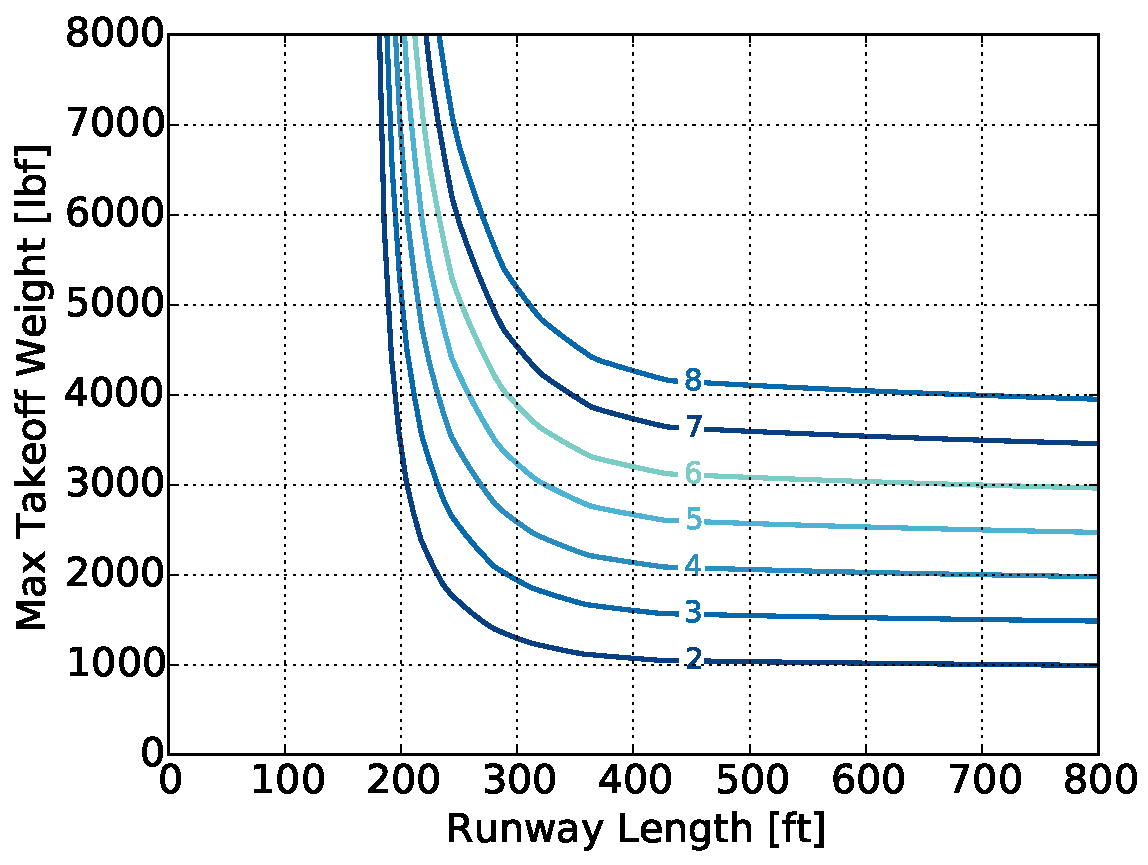
\includegraphics[]{sw_mtow.pdf}}
     \subfigure[\label{f:sw_mtowsens}Sensitivity to landing constraints]{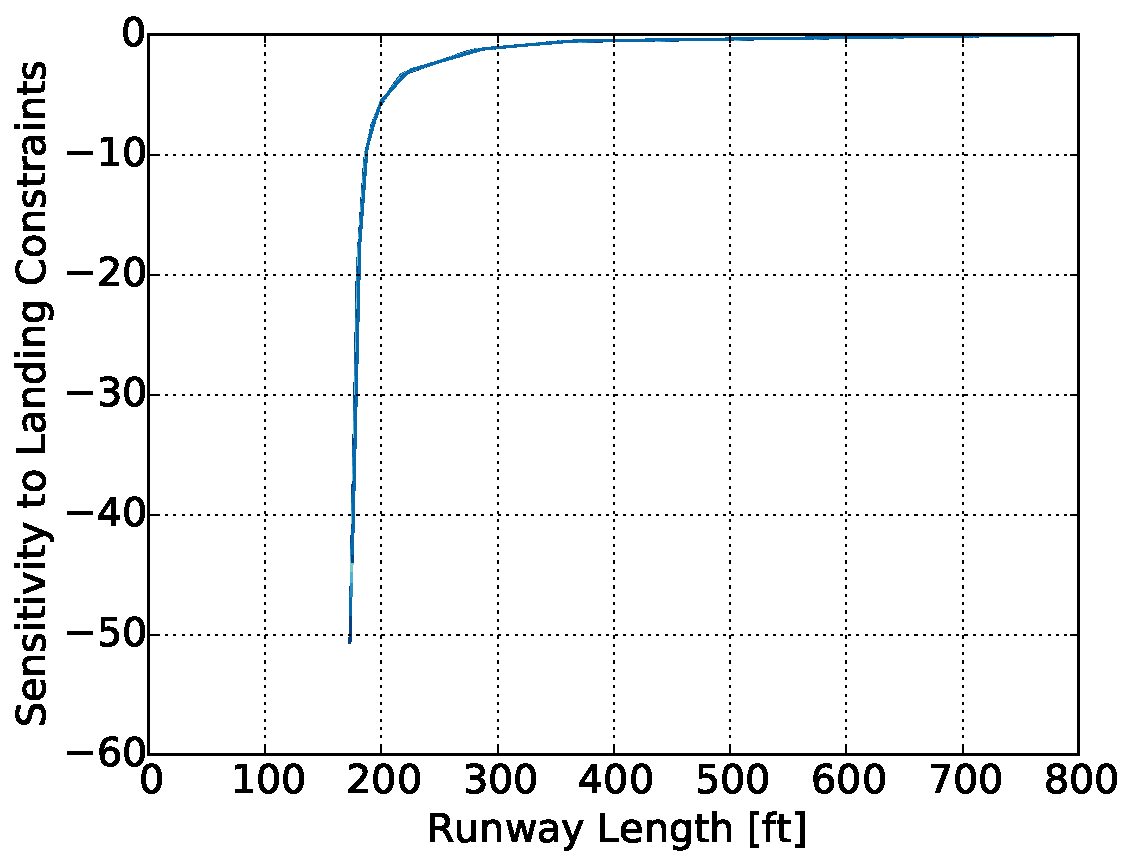
\includegraphics[]{sw_mtowsens.pdf}}
 \end{subfigmatrix}
    \caption{\textbf{Trade space of aircraft weight, number of passengers and runway length.}}
 \label{f:sw_mt}
\end{figure}

By looking at the sensitivity to the lift coefficient, shown in figure~\ref{f:sw_mtowsens}, on landing for the same trade study shown in figure~\ref{f:sw_mtow}, it can be determined whether the aircraft is constrained by the landing constraints or the take off constraints. 
The sensitivity to a variable in a geometric program is defined as the percentage change in the objective function for a 1\% change in that variable's value.  
For this study, either the landing constraints or the take off constraints will be active or driving the size of the vehicle.  
Thus, if the sensitivity to the lift coefficient on landing is zero, then the landing constraints are not active. 
Conversly, if the sensitivity is non-zero then those constraints are active and the vehicle size is landing constrained. 

Another way to view this trade space is to understand how runway length and range are effected by different minimum speed requirements.  
Figure~\ref{f:minspeed} shows plots of minimum cruise speed vs max take off weight for different contours of runway length and range requirements.  
This trade study was done for 5 passengers.  
These plots show that short runway and longer range requirements are possible but require slower cruise speeds.  
Because power scales with velocity cubed, slower speed reduces the required power and therefore battery weight, which improves the whole system. 
Note that in both plots shown in figure~\ref{f:minspeed}, lowering the minimum speed does not always improve the vehicle weight.  
A flat curve indicates that the aircraft is not constrained by the minimum cruise speed because of the optimum cruise speed for that set of requirements is faster than the minimum cruise speed. 

\begin{figure}[h!]
 \begin{subfigmatrix}{2}% number of columns
     \subfigure[\label{f:vweightR}Contours of range]{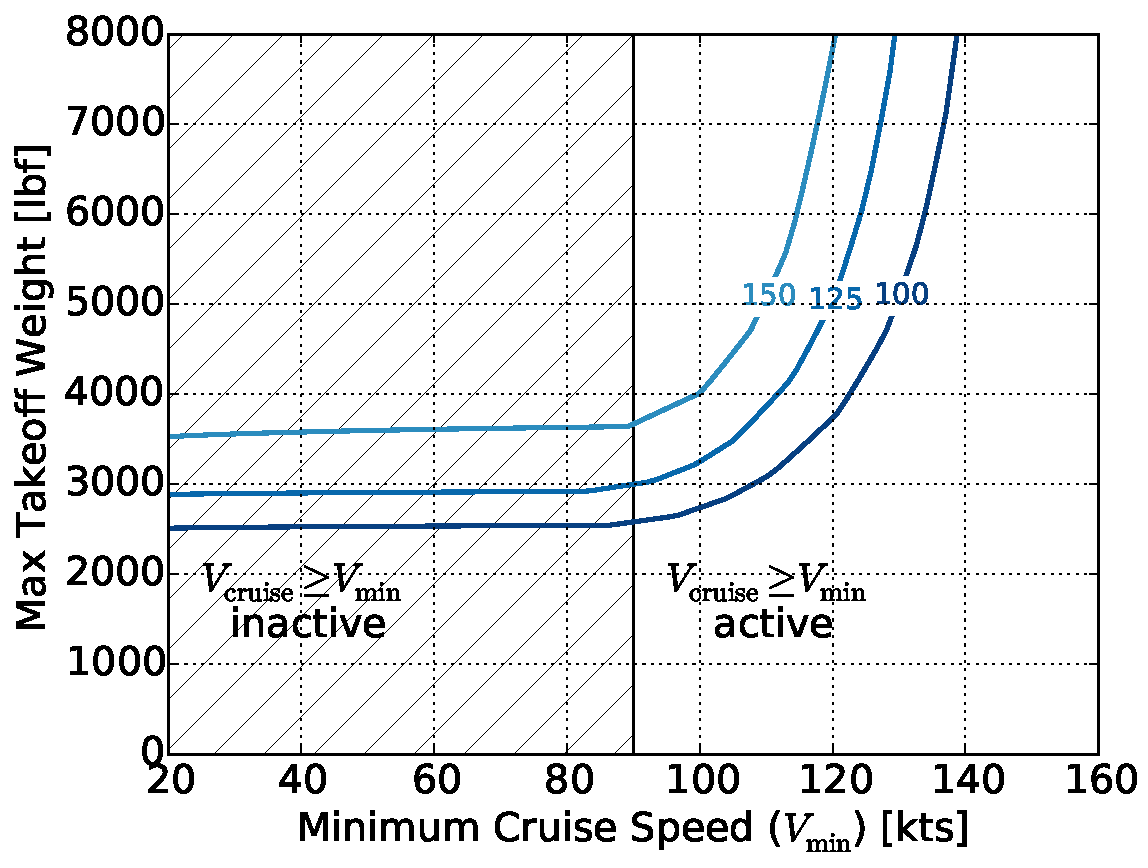
\includegraphics[]{vweightR.pdf}}
     \subfigure[\label{f:vweightS}Contours of runway length]{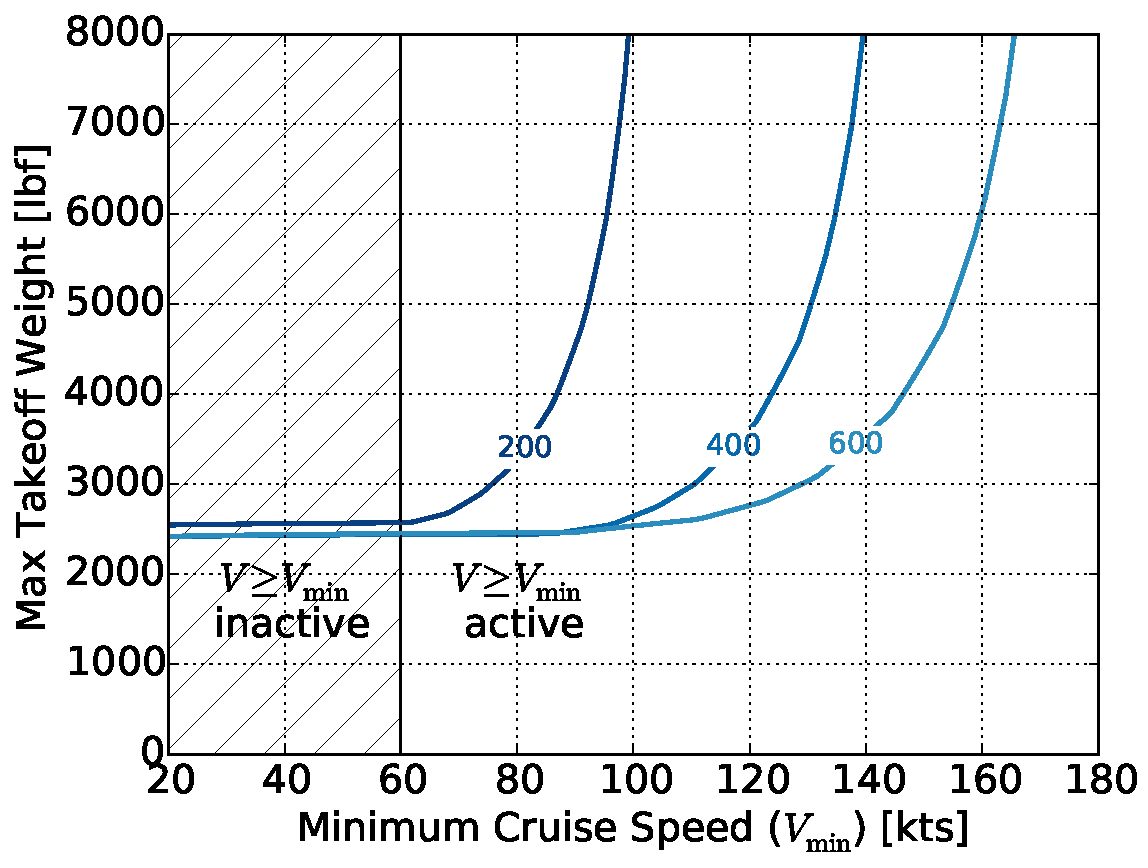
\includegraphics[]{vweightS.pdf}}
 \end{subfigmatrix}
 \caption{\textbf{Trade study between requirements of runway length, minimum speed and range.}}
 \label{f:rangetod}
\end{figure}

\subsection{Advanced Technology Trade Studies}

The previous section showed fundamental trade studies and trends for how runway length varies with performance.  
It is also possible to shorten runway length through advanced technology. 
As disscussed previously, a number of technologies could help reduce the required runway length including power bursts from electric motors, reverse thrust on landing, advanced flight controls, and improved battery technology.  
The effect of these technology advances on required runway length can be observed by changing a few parameters from the baseline case and resolving the optimization model.
Table~\ref{t:techparams} compares the baseline parameters to the advanced technology parameters that were assumed in the optimization model. 

\begin{table}[H]
    \centering
    \caption{Advanced Technology Parameter Assumptions}
    \label{t:techparams}
    \begin{tabular}{l c c}
    \toprule
    \toprule
    Parameter                         & Baseline Value  & Advanced Value \\ \hline
    $h_{\mathrm{batt}}$               & 210 [Whr/kg]    & 300 [Whr/kg]   \\
    $P_{\mathrm{spec}}$               & 0.7136 [kW/N]   & 0.571 [kW/N]   \\
    $C_{L_{\mathrm{max}}}$ (Landing)  & 3.5             & 4.5            \\
    $C_{L_{\mathrm{max}}}$ (TO)       & 4.0             & 5.0            \\
    $N$                               & 0.3             & 0.5            \\
    Runway margin                     & 40\%            & 20\%           \\
    Stall speed margin                & 30\%            & 10\%           \\
    \bottomrule
\end{tabular}
\end{table}

The motor power to weight ratio was lowered to take credit for the electric motor power burst during take off and is 80\% of the baseline value. 
The maximum lift coefficient during landing and takeoff were increased to match values predicted by NASA.
The landing deceleration factor was increased to take credit for use of reverse thrust on landing.
The lower margins on the runway length and stall speed are assuming advanced flight controls that require less margin. 
Realistically achieving all of these advances in a STOL aircraft design is unlikely.  
However, understanding the extremes between the baseline, conservative case and a more optimistic case is useful in determining a feasible vehicle design and vehicle requirements. 
Figure~\ref{f:sw_mtt} shows the same trade study as figure~\ref{f:sw_mt}, but with the updated parameter values shown in Table~\ref{t:techparams}.

\begin{figure}[h!]
 \begin{subfigmatrix}{2}% number of columns
     \subfigure[\label{f:sw_mtowt}Contours of number of passengers]{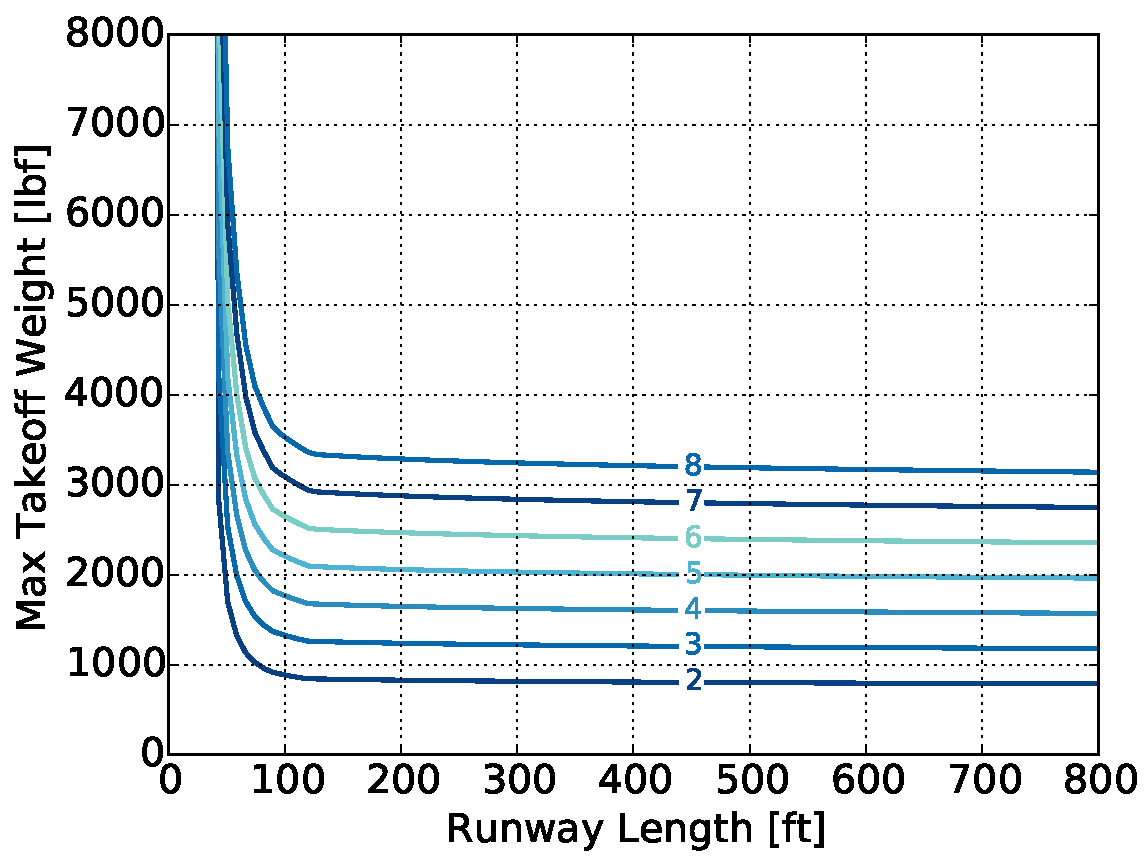
\includegraphics[]{sw_mtowt.pdf}}
     \subfigure[\label{f:sw_mtowtsens}Sensitivity to landing constraints]{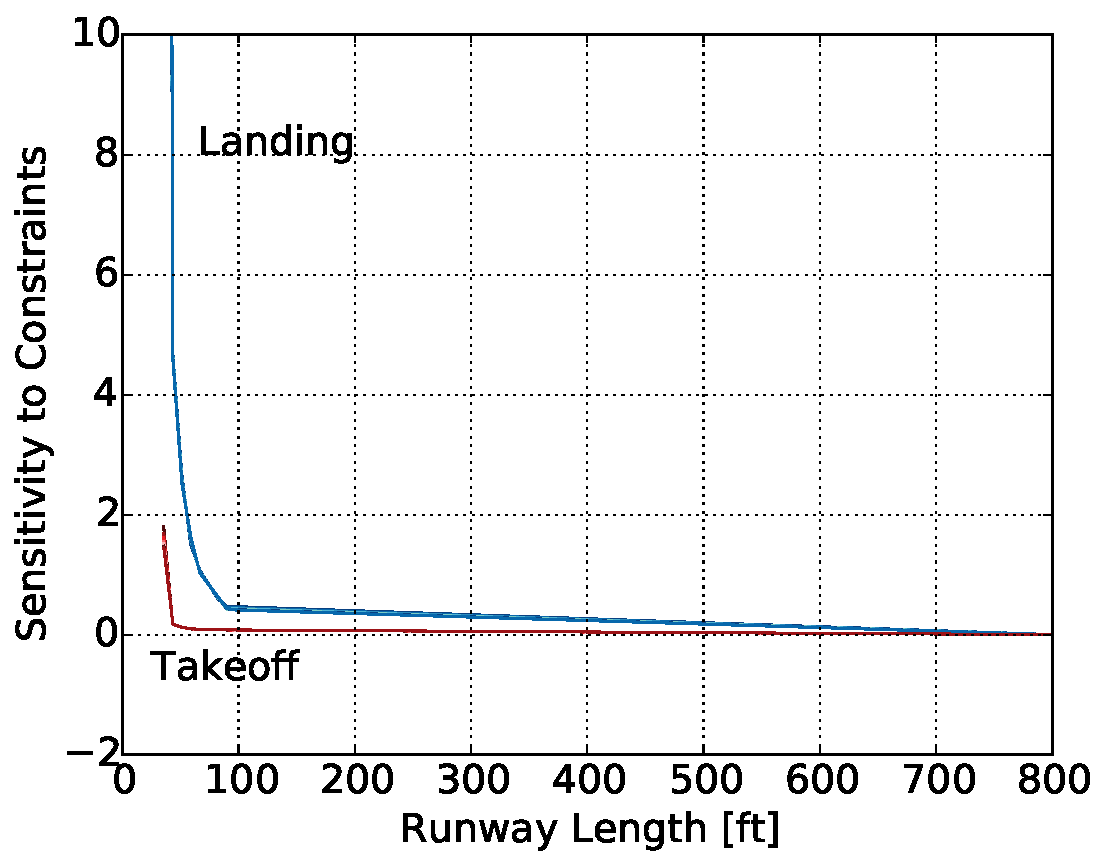
\includegraphics[]{sw_mtowtsens.pdf}}
 \end{subfigmatrix}
    \caption{\textbf{Trade space of aircraft weight, number of passengers and runway length for advanced technology assumptions.}}
 \label{f:sw_mtt}
\end{figure}

As observed in figure~\ref{f:sw_mtowt}, the advanced techonology assumptions allow for a much shorter runway than the baseline case showing that runways below even 100 ft might be possible. 
To understand which parameters have the largest effect on this trade study, each parameter can be varied one at a time from the baseline case. 
Figure~\ref{f:tech} show variations on the 5 passenger contour from figure~\ref{f:sw_mtow}. 

\begin{figure}[h!]
 \begin{subfigmatrix}{3}% number of columns
     \subfigure[\label{f:smtow_clmax}Contours of $C_{L_{\mathrm{max}}}$]{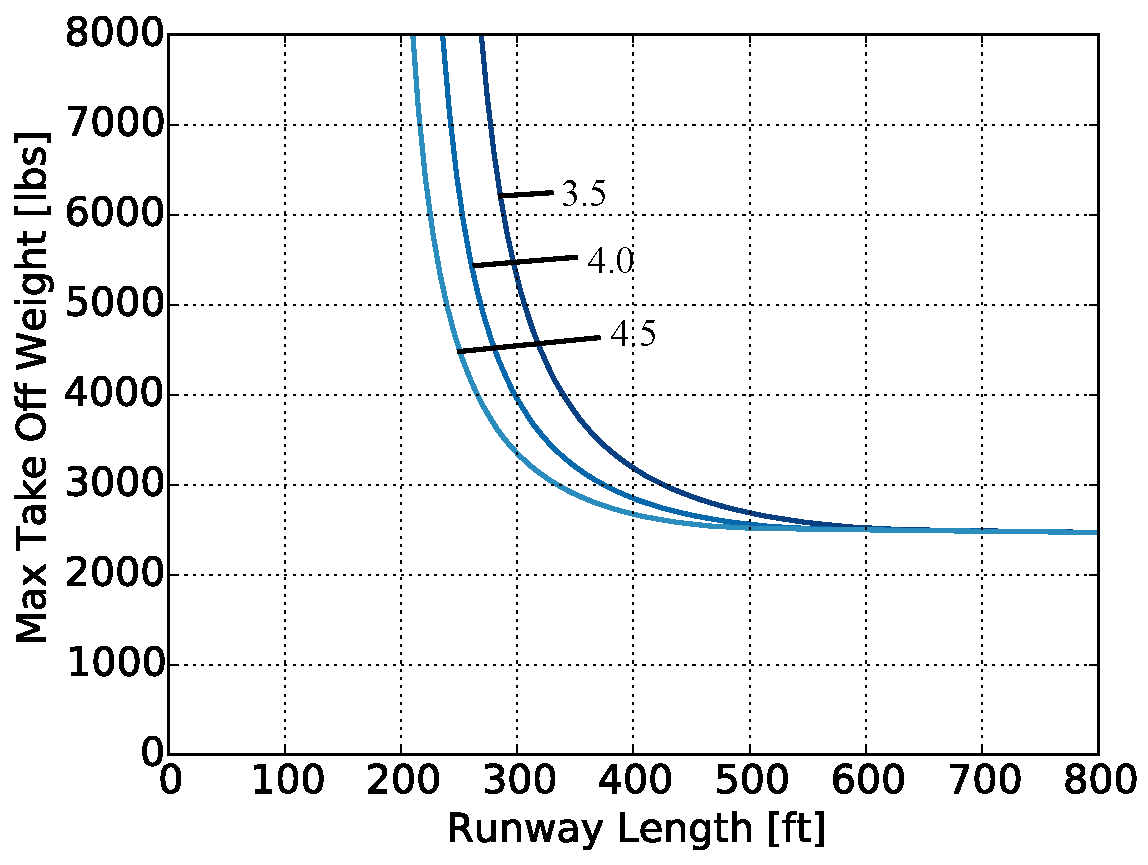
\includegraphics[]{smtow_clmax.pdf}}
     \subfigure[\label{f:smtow_gl}Contours of deceleration factor]{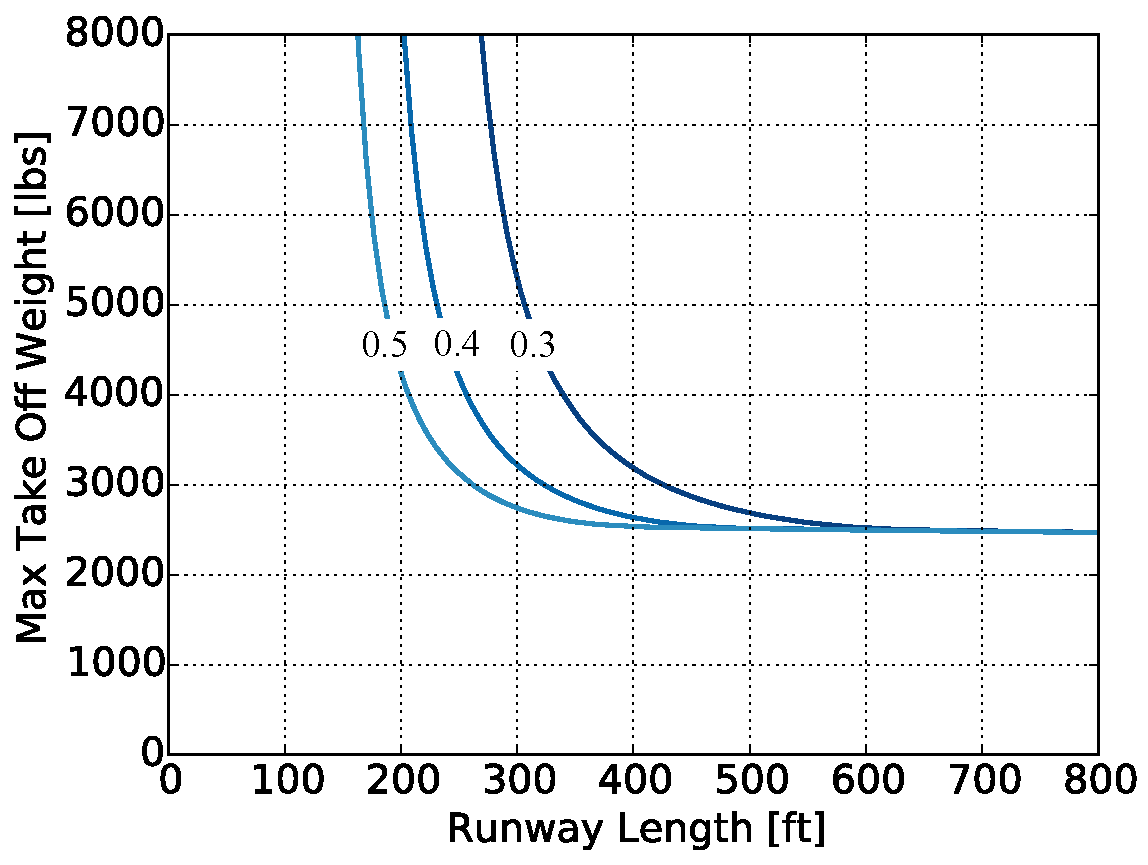
\includegraphics[]{smtow_gl.pdf}}
     \subfigure[\label{f:smtow_hbatt}Contours of battery specific energy]{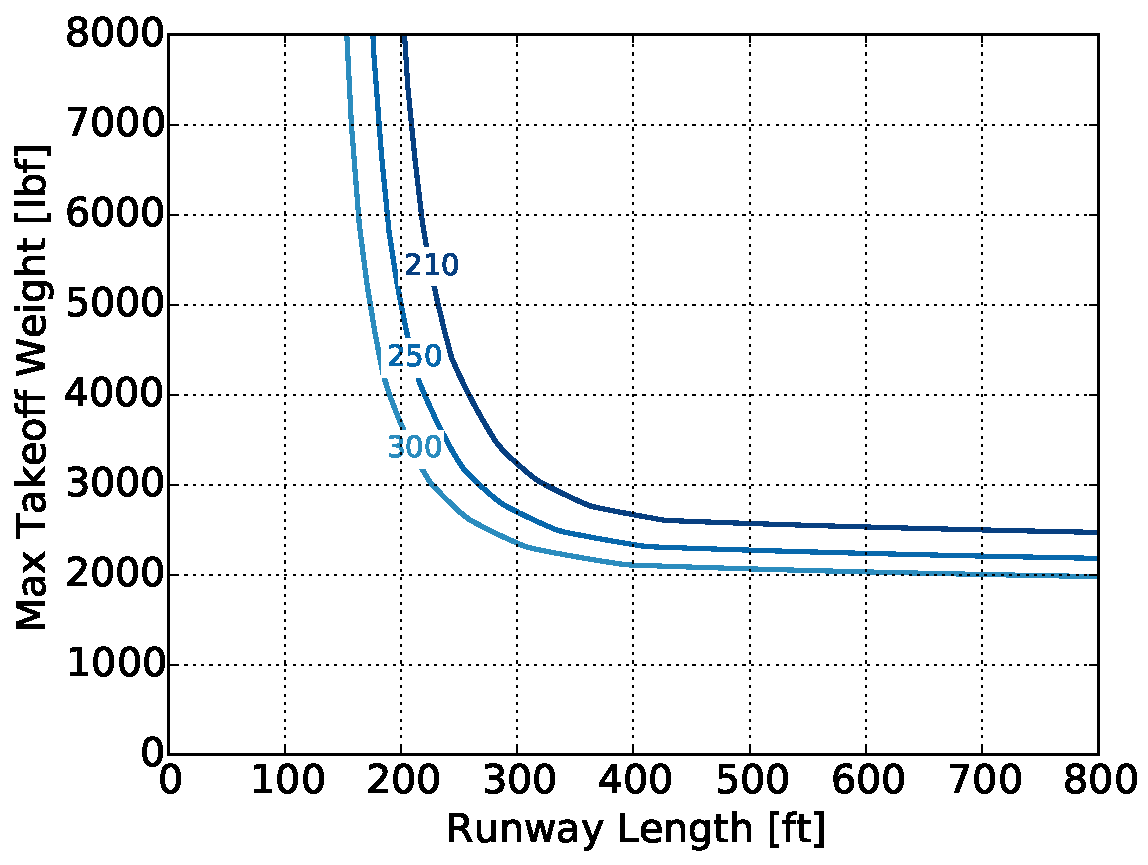
\includegraphics[]{smtow_hbatt.pdf}}
 \end{subfigmatrix}
    \caption{\textbf{Trade space of aircraft weight, number of passengers and runway length for advanced technology assumptions.}}
 \label{f:tech}
\end{figure}

Note that increasing the maximum lift coefficient or the deceleration factor has no effect for higher runway lengths.  
This is because at higher runway lengths the size of the aicraft is constained by the range requirement but not the runway requirement. 
Increasing the battery specific energy however, is always beneficial because that lowers the battery weight which improves the whole system. 

\section{Infrastructure}
Infrastructure is another aspect of the system that drives the vehicle design. A range of feasible runway lengths is a requirement that flows from infrastructure and in turn defines what vehicle designs are also feasible. As previously discussed, there is a substantial amount of airport infrastructure located outside of urban centers; however within an urban center, much less airport or runway infrastructure exists. Therefore this infrastructure study will specifically consider feasible infrastructure within an urban center. The city of Boston will be used for this case study. Key topics to address include what considerations drive the placement of STOLports, what are feasible location types, and how does infrastructure availability change with infrastructure type and required size. The goal in selecting locations for STOLport infrastructure is to be able to connect to existing transportation infrastructure within an urban center.
\paragraph{Site Considerations}
Site considerations are not driven solely by runway length. The minimum rectangular area upon which a STOLport can be built is defined by runway length as we well as room for taxiways, clearway requirements, and space for parking and charging stations. Clearway requirements are written in the FAA AC 150/5300 and are dependent on aircraft size and speed [1???]. For locations that may be space restricted, a STOLpad rather than a STOLport concept is possible, which would consist of only the bare minimum infrastructure and would not include space for considerations such as parking and charging stations. Site considerations are also dependent on VFR approach and departure paths and the need for obstacle avoidance. Obstacle avoidance is defined as a plane of a defined width at a given distance and height from the runway, through which no obstacle may protrude; obstacle avoidance definitions are also dependent on vehicle size and speed [1???]. The key drivers for site considerations are area available, which is more than solely runway length, and obstacle avoidance for approach and departure paths.
\paragraph{Crosswing Mitigation}

An additional consideration for infrastructure availability is crosswind mitigation. In order to have a robust UAM system, wind should not be a prohibitive factor for operations. Specific considerations for the particular wind patterns of the city in question should be incorporated when deciding on infrastructure location. There are various techniques to mitigate for multiple wind directions. One way is to have conventional crosswind runways. A disadvantage for this is that it will require additional surface area for the STOLport, which could possibly reduce the amount of infrastructure available. To reduce the severity of this impact, the crosswind design could take credit for the headwind component inherent in triggering the switch to the crosswind runway. A rule of thumb says that take-off and landing distances are reduced by 1.5 $\%$  for each knot of headwind up to 20 knots [experimentalaircraft.info reference]. An additional option would be to create a circular STOLport with the diameter of the required runway length. The runway heading could be set dynamically based on the prevailing winds. This would require more complex approach and departure procedures, 360-degree obstacle clearance, and portable charging stations. If the STOLport is built over linear pre-existing infrastructure such as highways and railways, an additional STOLport can be built nearby with a perpendicular orientation to serve the same geographic location when crosswind conditions exist. Lastly, if barges are used as the STOLport then they could be moored to allow for rotation into the wind. This would require an increased footprint in the waterways which needs to be deconflicted with boating channels.
In addition to infrastructure design, the eSTOL vehicle design could also be used to mitigate crosswind landings. A larger vertical stabilizer or increased control surface could increase the safe crosswind strength on landing. The design could also incorporate specific adjustments to the landing gear to facilitate higher crosswind landings, such as rotating landing gear, which would allow the nose of the aircraft to remain into the wind all the way through touchdown. One additional design consideration would be to introduce advance controls or maneuvers to allow for safe crosswind landings. With advances happening rapidly with high-precision approach and landing guidance, crosswind landings can be mitigated through automation.

\paragraph{Feasible Locations}
A network of notional sites within Boston was designed with the previous considerations in mind. The network of notional sites is shown in Figure ~\ref{f:nsites}. Within the network there are four types of possible STOLport locations, which are also shown in Figure ~\ref{f:nsites}. The four types of locations to place a STOLport are on top of a building, over a highway or railway, on a barge over a body of water, or on the ground. Visualizations for the four types of STOLport locations are shown in Figure ~\ref{f:svis}. The barge location shows a runway and possible space for charging stations.  The highway or railway location shows a runway on an elevated structure, with a ramp for the aircraft to taxi down to a lower level with charging stations. The building location shows the possibility for crosswind runways depending on the are available, and space for charging stations are also shown. The ground location is similar to the building location with crosswind runways depending on the area available and charging stations again shown. The network of notional sites identified accounting for previously discussed considerations included building locations, highway or railway locations, barge locations, and ground locations.
\begin{figure}[h!]
	\begin{center}
	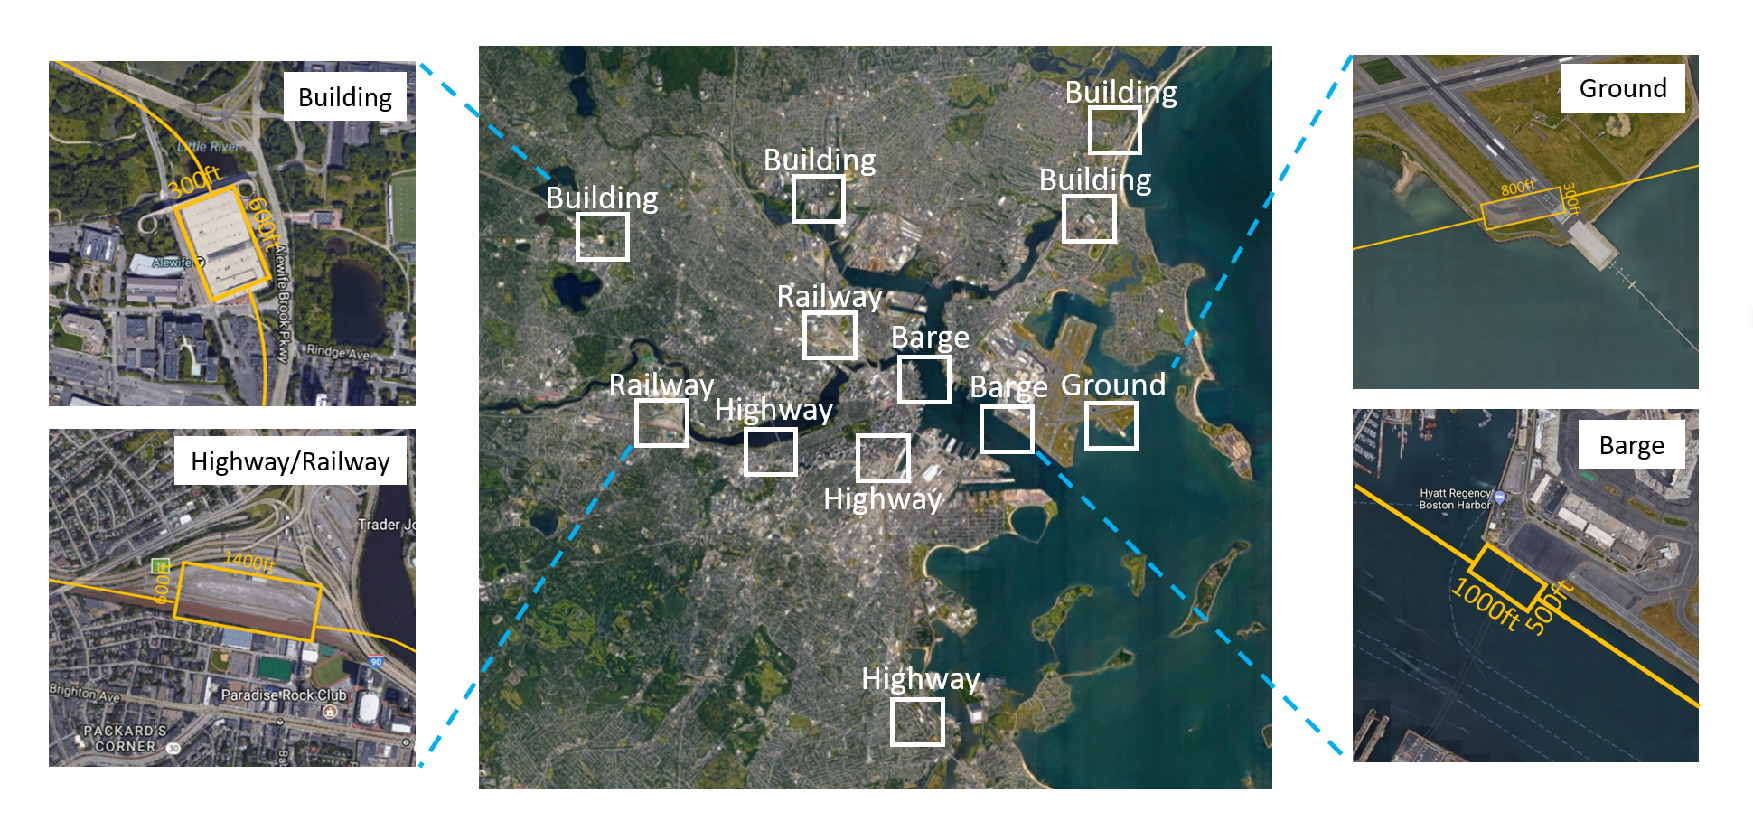
\includegraphics[width=1.0\textwidth]{2 Notional Sites.pdf}
    \caption{\textbf{Notional sites for STOLport locations}}
	\label{f:nsites}
	\end{center}
\end{figure}
\begin{figure}[h!]
	\begin{center}
	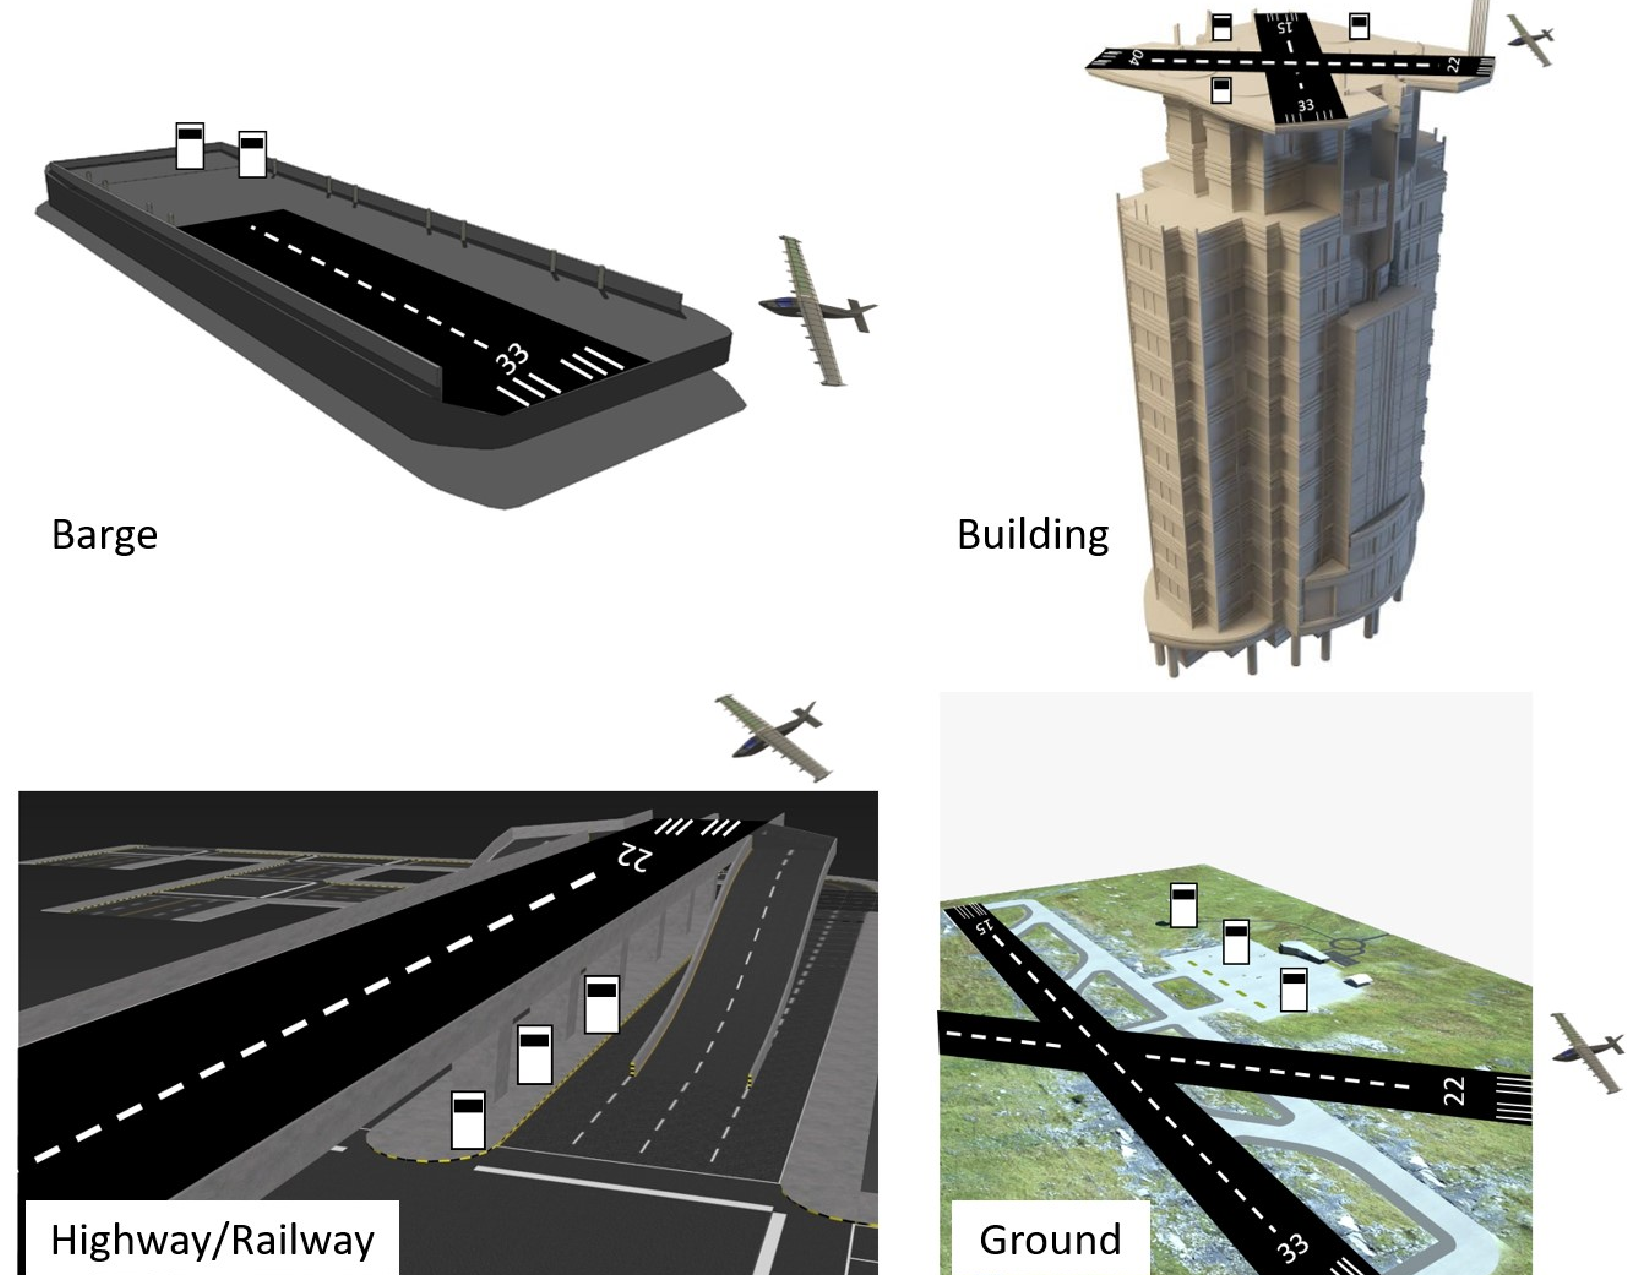
\includegraphics[width=1.0\textwidth]{3 STOLport Visualizations.pdf}
    \caption{\textbf{STOLport placement options}}
	\label{f:svis}
	\end{center}
\end{figure}
\paragraph{Scaling}
Considerations for scaling an infrastructure network vary depending on the type of STOLport location. At highway and railway locations, placing any length of runway is fairly easy because the length of highways and railways far exceeds the length of STOLport runways; however the amount of above ground highway and railway infrastructure is limited in downtown areas due to tunnels. Many major cities are located by large bodies of water which allows for much area in order to scale the number of barge locations; however barges must consider ways to connect to the shore and avoiding shipping lanes. Scaling a network of ground infrastructure locations is not really feasible in an urban center aside from already existing airports. Buildings are generally widely available within an urban center, however buildings will require shorter runway lengths than some of the other locations. Building STOLport locations are the type of location that is most dependent on runway length.
	In order to understand how building infrastructure varies with runway length, heat maps and histograms were created. Figure ~\ref{f:heatmap} shows heat maps for Boston and Los Angeles. The data used is GIS data and possible buildings were defined such that the building footprint had at least one dimension that was as long as the runway length [2,3]. The heat maps show that the possible buildings for different runway lengths are distributed throughout the city making it possible to scale an infrastructure network that is not all concentrated at one location. The building histograms in Figure ~\ref{f:hist} provide insight into how the number of available buildings varies with runway length. Runway lengths of approximately 400-600 feet do allow for a feasible number of building locations to design a network, and runway lengths of 300 feet or less allow for a significant increase in the number of possible building locations. The trend is that as runway length increases, the number of available buildings exponentially decreases.
\begin{figure}[h!]
	\begin{center}
	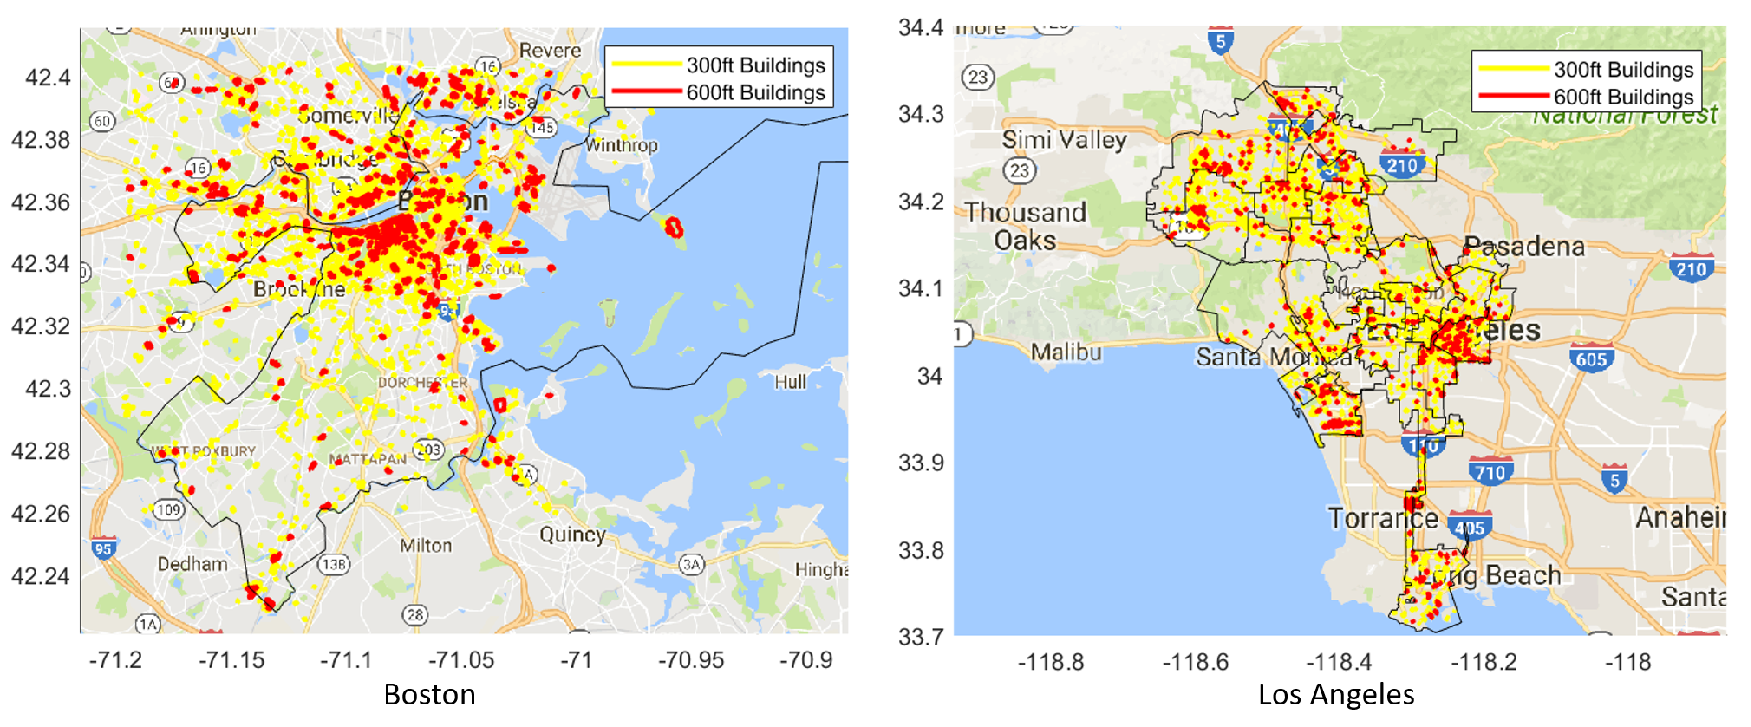
\includegraphics[width=1.0\textwidth]{4 Building Heat Maps.pdf}
    \caption{\textbf{Notional sites for STOLport locations}}
	\label{f:heatmap}
	\end{center}
\end{figure}
\begin{figure}[h!]
	\begin{center}
	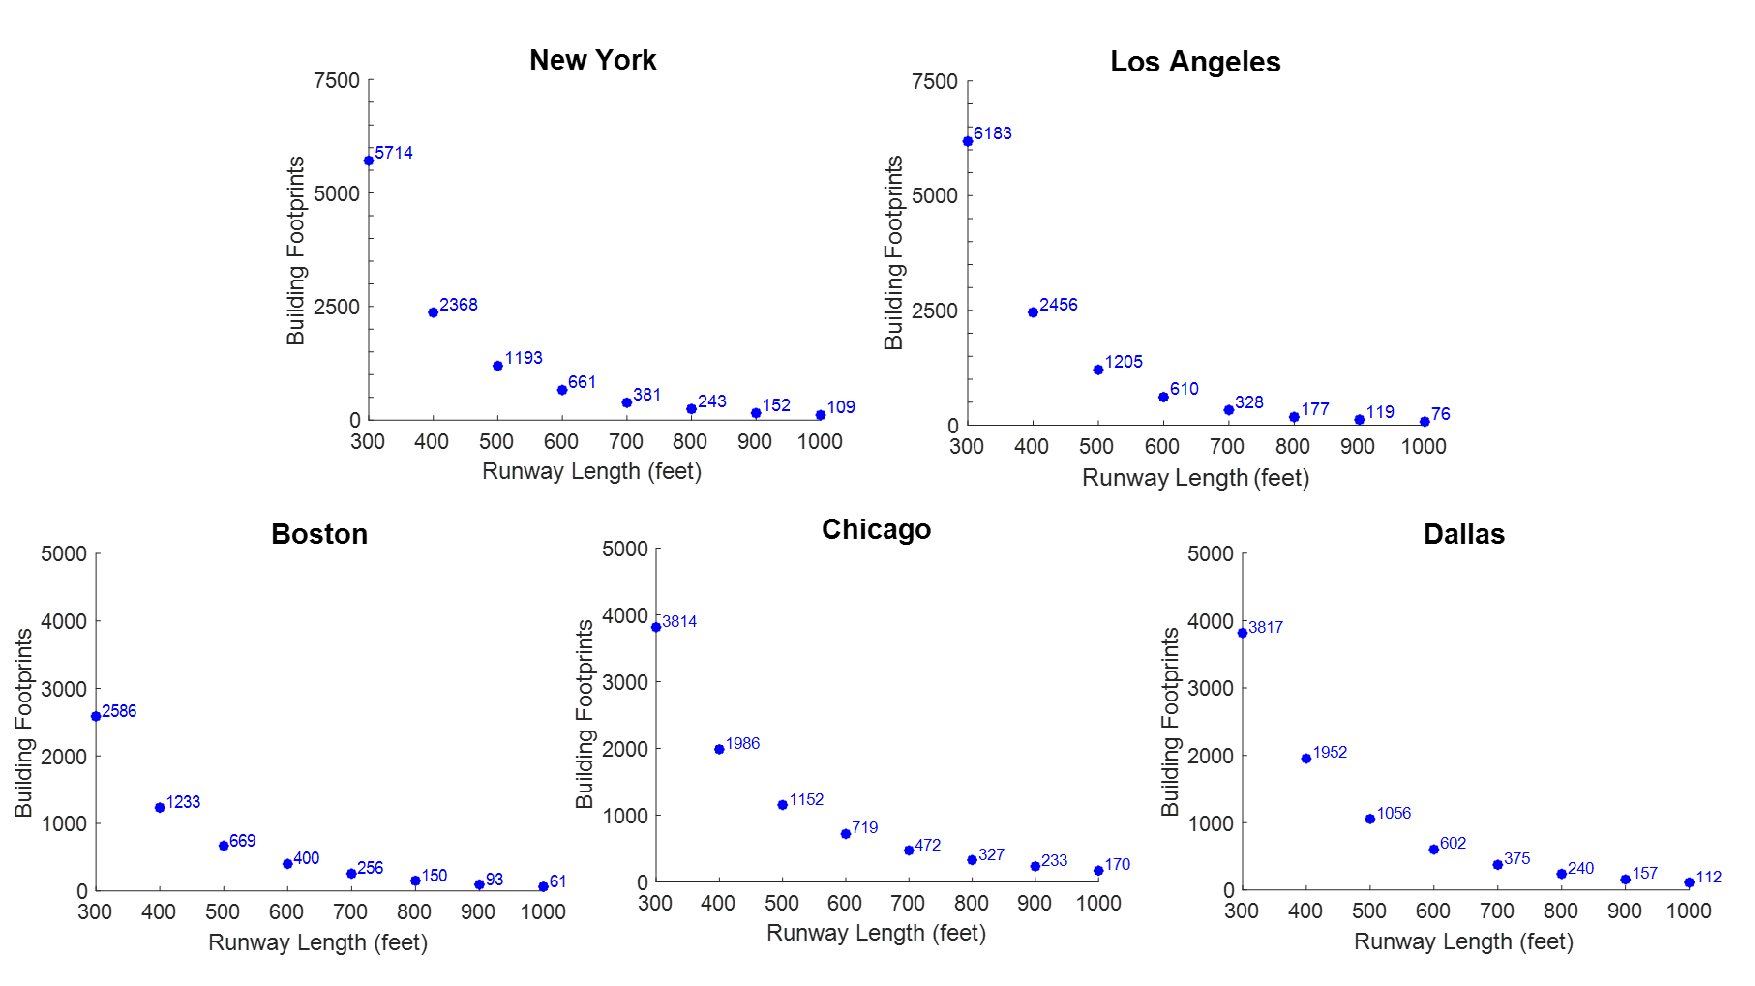
\includegraphics[width=1.0\textwidth]{5 Building Histograms.pdf}
    \caption{\textbf{STOLport placement options}}
	\label{f:hist}
	\end{center}
\end{figure}

\section{Conclusion}
\paragraph{Infrastructure}
Possible types of locations for STOLports identified in this study include on top of buildings, over highways and railways, on barges, or on the ground of existing airports. These locations can support runway lengths of 400 to 600 feet; if the STOL vehicle is able to land in a runway length of 300 feet or less, then the number of possible buildings significantly increases. Landing in a runway length of 500 feet or less could allow for novel operations at existing major airports. The results of the infrastructure study indicate that it is possible to design a STOLport network in an urban center.
\paragraph{Risks Revisited}

\bibliography{biblibrary}
\bibliographystyle{aiaa}

\end{document}

